\section{Calibrazione}
La calibrazione del ricevitore a 1.4 a GHz viene effettuata utilizzando due sorgenti di riferimento, che sono due carichi coassiali adattati, cioè due resistenze a 50 $\Omega$. Questi lavorano a due temperature diverse: uno a temperatura ambiente (\textit{warm load}) e l'altro alla temperatura di ebollizione dell'azoto liquido, ovvero 77,36 K (\textit{cold load}). \\\\Il carico a temperatura criogenica è connesso al ricevitore tramite un cavo coassiale il quale è immerso parzialmente nell'azoto liquido. Perciò, dato che la temperatura del cavo non è uniforme, ne vanno studiate le caratteristiche di attenuazione in laboratorio, su un cavo analogo, a temperatura ambiente ed a temperatura criogenica. Per farlo si utilizza un analizzatore vettoriale di reti (VNA).

\subsection{Attenuazione cavo coassiale}
Il cavo Cold Load che viene utilizzato nella calibrazione del ricevitore è solo parzialmente immerso nell'azoto liquido, la sua temperatura non è quindi costante. Perciò, il coefficiente di attenuazione del cavo viene misurato con il VNA sia a temperatura ambiente, sia a temperatura criogenica. Per farlo si utilizza un cavo di rame analogo di forma elicoidale, così da facilitarne l'immersione nell'azoto, e di lunghezza 203 cm. 
\begin{figure}[h]
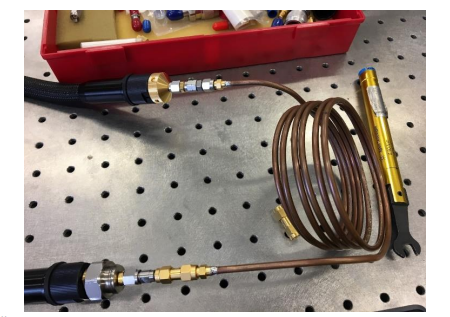
\includegraphics[scale=0.60]{cavo rame.png}
\centering
\caption{Cavo di rame collegato alle porte del VNA}
\label{fig:Cavo di rame}
\end{figure}

Il rame, però, ha una conducibilità termica molto elevata. Per questo motivo, al fine di prottegere il VNA ed evitare che i suoi cavi lavorino ad una temperatura di 77,36 K, si utilizzano dei separatori termici. Essi stessi tuttavia attenuano il segnale. Viene quindi effettuata una misura intermedia dell'attenuazione dei separatori, collegandoli tra loro. In questo modo è poissibile togliere il loro contributo dal calcolo del coefficiente di attenuazione del cavo di rame.
\subsubsection{VNA e parametri di scattering}
Il VNA è una macchina che permette di misurare le proprietà di trasmissione di un cavo coassiale i cui estremi sono connessi ai terminali dello strumento. Il VNA presente il laboratorio è un Agilent PNA-X che è in grado di misurare in modo indipendente il segnale di trasmissione e riflessione dalle due porte presenti.
\begin{figure}[h]
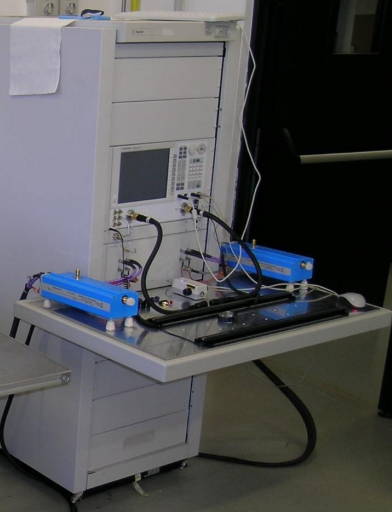
\includegraphics[scale=0.60]{VNA.png}
\centering
\caption{VNA presente in laboratorio. Il modello è un Agilent PNA-X.}
\label{fig:VNA}
\end{figure}

Quindi ciò che la macchina restituisce è la cosiddetta matrice di scattering i cui parametri sono: i coefficienti di riflessione, \textit{$s_{11}$} e \textit{$s_{22}$}, ed i coefficienti di trasmissione, \textit{$s_{12}$} e \textit{$s_{21}$}. Dove vale che:\\\\
\begin{equation}
    s_{11}=10\log_{10} \frac{Potenza\,\,riflessa\,\,nella\,\,porta\,\,1}{Potenza\,\,incidente\,\,dalla\,\,porta\,\,1}
\end{equation}
\begin{equation}
    s_{12}=10\log_{10} \frac{Potenza\,\,trasmessa\,\,dalla\,\,porta\,\,1\,\,alla\,\,porta\,\,2}{Potenza\,\,incidente\,\,dalla\,\,porta\,\,1}
\end{equation}
\begin{equation}
    s_{21}=10\log_{10} \frac{Potenza\,\,trasmessa\,\,dalla\,\,porta\,\,2\,\,alla\,\,porta\,\,1}{Potenza\,\,incidente\,\,dalla\,\,porta\,\,2}
\end{equation}
\begin{equation}
    s_{22}=10\log_{10} \frac{Potenza\,\,riflessa\,\,nella\,\,porta\,\,2}{Potenza\,\,incidente\,\,dalla\,\,porta\,\,2}
\end{equation}
\\NON SO SE METTERE QUESTA PARTE
Impostiamo che la macchina lavori in una banda di frequenza che varia dai 500 MHz ai 3 GHz e che faccia una scansione in frequenza in 201 punti e con una potenza di 0 dB. Per calibrare la macchina è necessario togliere l’effetto dei cavi di misura: per farlo si danno, tramite calibratore elettronico, degli standard di riferimento: lo standard di riflessione totale e lo standard di trasmissione e di sfasamento. In questo modo viene calcolato l’error box della macchina, cioè la matrice di compensazione dell’effetto dei cavi.


\subsubsection{Matrice di scattering con separatori termici}
\subsubsection{Matrice di scattering con separatori termici e cavo di rame}
\subsubsection{Matrice di scattering del cavo di rame}
\subsubsection{Calcolo del coefficiente di attenuazione}


\subsection{Calibrazione del ricevitore a 1.4 GHz}
\subsubsection{Profilo di temperatura del cavo}
\subsubsection{Temperatura del cavo cold load}
\subsubsection{Temperatura del cavo warm load}
\subsubsection{Guadagno del ricevitore}
\subsubsection{Temperatura di rumore}